\chapter{Solides de l'espace}
%\stepcounter{module}

{\AlegreyaSansLight \large
\begin{center}
\textbf{Crédit :} 11 heures\\
\textit{4 heures hebdomadaires}
\end{center}
}

\minitoc

\section{Introduction}

\subsection{Présentation du module}
Ce module comporte deux parties essentielles : prismes droits et sphère. Il développe deux compétences fondamentales que sont :
\begin{itemize}
\item déployer un raisonnement mathématique (analogique, inductif et déductif)
\item résoudre des problèmes par l'observation, l'identification et la caractérisation des objets de l'espace.
\end{itemize}
Il s'articule sur la famille de situations suivante : usage des objets techniques dans la vie. Les compétences mises en contexte s'appuient sur les trois catégories d'actions qui suivent :
\begin{itemize}
\item Reconnaissance des solides dans l'espace.
\item Production d'objets.
\item Détermination des mesures.
\end{itemize}
Cette dernière catégorie d'actions est le champ privilégié de l'inter action entre les activités numériques et les activités géométriques de l'élève de 5ème.\\
Les différentes actions qui s'intègrent dans chacune des catégories suscitées sont en corrélation avec les savoirs essentiels que ce module développe, et qui s'appuient sur les habiletés cognitives suivantes : connaissance, compréhension et application.
\subsection{Contribution du module à la finalité et aux buts curriculaires}
L'apprentissage de la géométrie en général, et de la géométrie dans l'espace en particulier concourt à la construction du raisonnement, à la familiarisation avec les techniques calculatoires telles que les calculs d'aires et des volumes. Le traitement de la famille de situations aidera l'élève à construire ces éléments de formation. Il pourra également se familiariser avec les techniques de classement, d'observation et de description, de représentation, autant d'attitudes qui contribuent à l'autonomie.
\subsection{Contribution du module au programme d'études et aux domaines de vie}
Les éléments de formation que l'élève construira en traitant avec compétence la famille de situations choisie devrait l'aider à réaliser des actions et résoudre des problèmes.\\
De plus, le présent module est d'un apport significatif au domaine d'apprentissage intitulé « sciences et technologie », tant il participe à la conception, à la représentation, et à la réalisation des chefs d'œuvres architecturaux, et de tous les objets technologiques qui nous entourent. Sa contribution à la représentation
de la structure cristalline de certains éléments de base en chimie mérite elle aussi d'être soulignée. Enfin il ne serait pas superflu de signaler sa contribution au développement des arts plastiques et graphiques, véhicules de grandes valeurs universelles telles que l'esthétique et l'harmonie.\\
La contribution de ce module au développement de la technologie vient d'être soulignée plus haut. L'importance du développement de la technologie n'est plus à démontrer dans la vie économique, et dans l'amélioration du bien être familial. On peut donc affirmer par voie de conséquence que la contribution de ce module à la vie sociale et familiale, et surtout à la vie économique est déterminante. Cette contribution peut même être étendue, de manière implicite au domaine de la citoyenneté, et à celui des arts.

\section{Matrice}

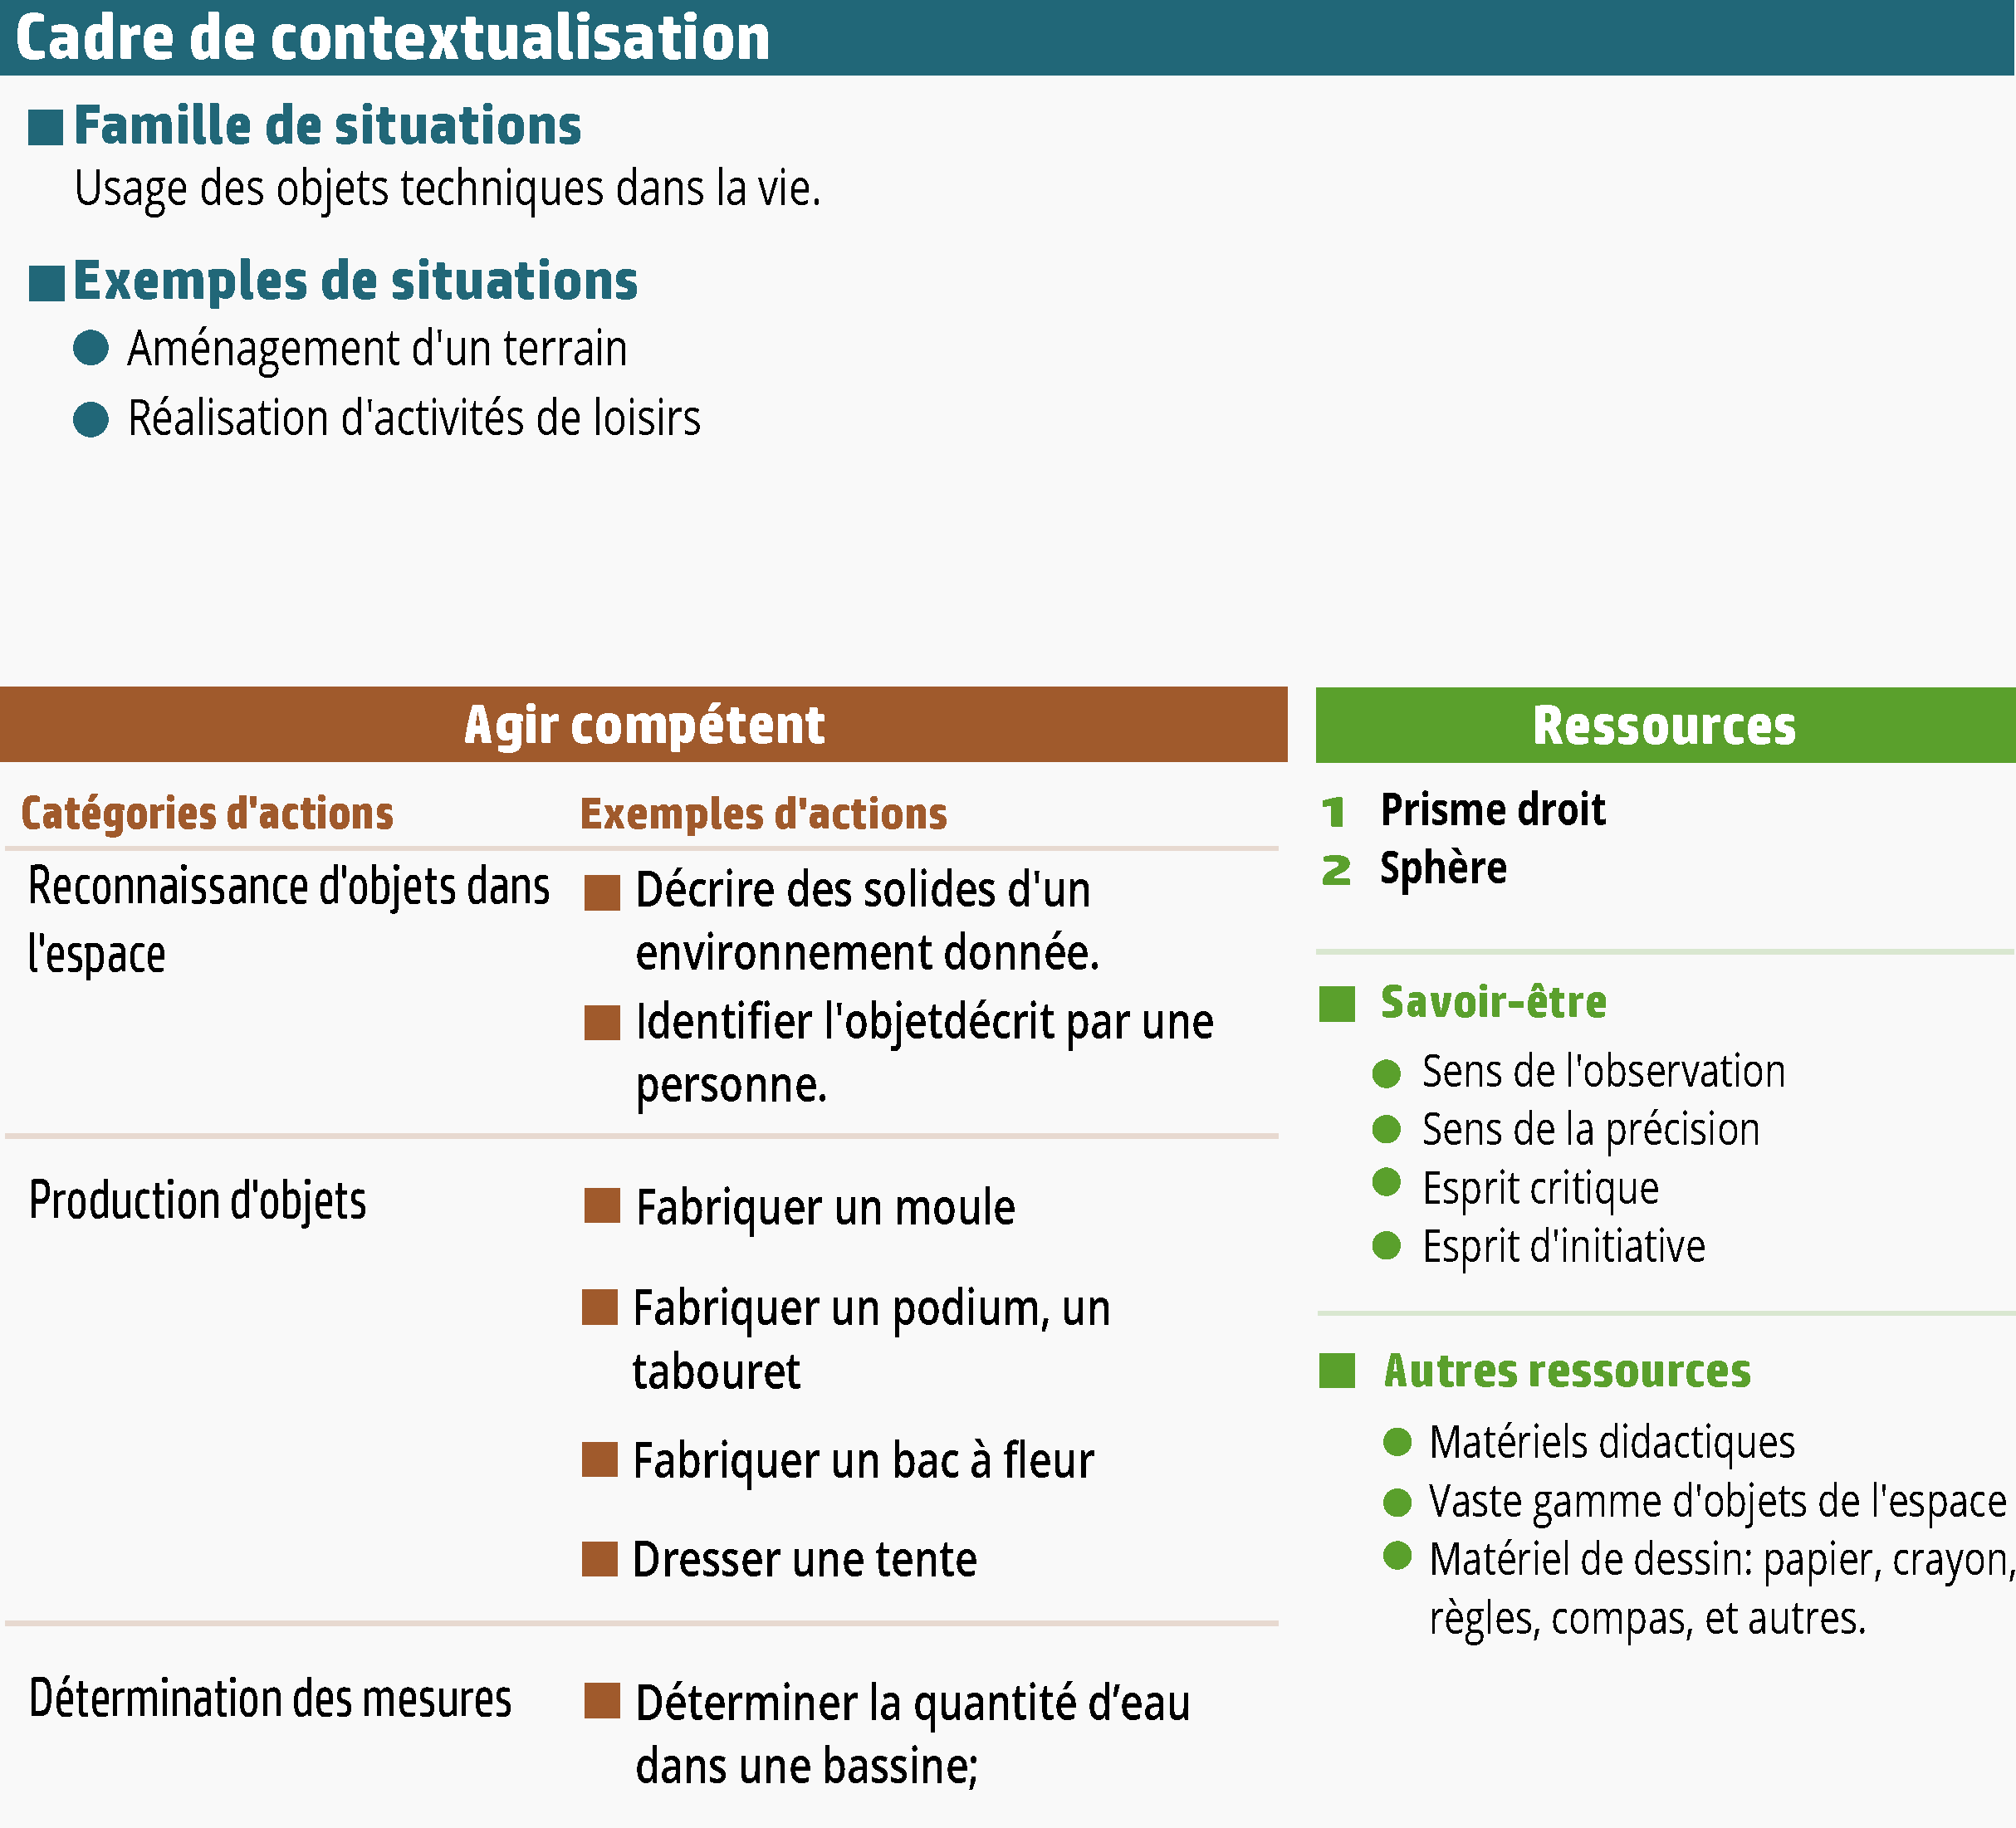
\includegraphics[width=\textwidth]{Module8.pdf} 

\subsection*{}
\addcontentsline{toc}{subsection}{\textbf{Ressource 1}: prisme droit}
\ressource{Pri.pdf}

\savoir
\begin{itemize}
\item \textit{Prisme droit} : forme, faces, bases, arêtes ;
\item \textit{Propriétés}: nombre de faces, d'arêtes, de sommets,
\item \textit{Eléments métriques}: aire latérale, aire totale, volume.
\end{itemize}
\savoirfaire
\begin{itemize}
\item Fabrication d'un prisme droit et réalisation d'un patron d'un prisme droit;
\item Calcul des éléments métriques (l'aire de la surface latérale, l'aire
totale, volume) ;
\end{itemize}

\newpage

\subsection*{}
\addcontentsline{toc}{subsection}{\textbf{Ressource 2}: sphère}
\ressource{Sph.pdf}

\savoir
\begin{itemize}
\item Sphère et boule : forme, centre, rayon, diamètre;
\item Eléments métriques : aire d"une sphère et volume d'une boule.
\end{itemize}
\savoirfaire
\begin{itemize}
\item Calculs sur les éléments métriques d'une sphère/boule (aire d'une sphère et volume d'une boule, rayon).
\end{itemize}